\documentclass[10pt]{beamer}

\usetheme[numbering=fraction,block=fill]{metropolis}

\usepackage{appendixnumberbeamer}
\usepackage{booktabs}
\usepackage[scale=2]{ccicons}
\usepackage{listings}
\lstdefinelanguage{Julia}{
  morekeywords={using}, 
  sensitive=false,
  morecomment=[l]{\#},
  morestring=[b]", 
}
\lstset{ % General setup for the package
    language=Julia,
    basicstyle=\small\sffamily,
    numbers=left,
    numberstyle=\tiny,
    frame=tb,
    framerule=1pt,
    commentstyle=\color{teal},
    keywordstyle=\color{magenta}
}

\usepackage[absolute,overlay]{textpos}
\setlength{\TPHorizModule}{\paperwidth}
\setlength{\TPVertModule}{\paperheight}

% ------------------------ %
% 	  Packages		%
% ------------------------ %

\usepackage[utf8]{inputenc}
\usepackage[T1]{fontenc}
\usepackage{xcolor}
\usepackage[setbb,setcolon]{kmath}
\usepackage{xparse,pgffor,ifthen}
\usepackage{amsmath,amssymb,amsfonts,amsthm,mathrsfs,mathtools,bbm,stmaryrd}
\usepackage{tikz,pgfplots,forest}
\usepackage{cancel}
\usetikzlibrary{arrows.meta}
\pgfplotsset{compat=newest}
\usepgfplotslibrary{groupplots}
\usepackage[ruled,linesnumbered]{algorithm2e}
\usepackage{cleveref,csquotes,comment,lipsum,todonotes,soul,extarrows,graphicx}
\usepackage{glossaries}
\usepackage[numbers,sort&compress]{natbib}
\usepackage{glossaries,url,subcaption}
\usepackage[texcoord]{eso-pic}

\usepackage[most]{tcolorbox}
\newtcbox{\mytransparentbox}{blank, on line, opacitytext=0.4}

\usepackage{pifont}

% ------------------------ %
% 	  Shortcuts		  %
% ------------------------ %

% Lowercase styles
\foreach \x in {a,...,z}{%
	\expandafter\xdef\csname \x\endcsname{\noexpand\ensuremath{\noexpand\mathbf{\x}}}
}
\foreach \x in {a,...,z}{%
	\expandafter\xdef\csname \x rm\endcsname{\noexpand\ensuremath{\noexpand\mathrm{\x}}}
}

% Uppercase styles
\foreach \x in {A,...,Z}{%
	\expandafter\xdef\csname \x\endcsname{\noexpand\ensuremath{\noexpand\mathbf{\x}}}
}
\foreach \x in {A,...,Z}{%
	\expandafter\xdef\csname \x rm\endcsname{\noexpand\ensuremath{\noexpand\mathrm{\x}}}
}
\foreach \x in {A,...,Z}{%
	\expandafter\xdef\csname \x bb\endcsname{\noexpand\ensuremath{\noexpand\mathbb{\x}}}
}
\foreach \x in {A,...,Z}{%
	\expandafter\xdef\csname \x c\endcsname{\noexpand\ensuremath{\noexpand\mathcal{\x}}}
}

% Figures styles
\def\0{{\mathbf 0}}
\def\1{{\mathbf 1}}

% Miscellaneous
\def\ie{\emph{i.e.,}\xspace}
\def\eg{\emph{e.g.,}\xspace}
\def\etal{\emph{et al.}\xspace}
\def\resp{resp.\xspace}
\def\iif{iff.\xspace}
\def\st{\textsf{s.t.}\xspace}

% Notes
\def\addNote#1{{\noindent\color{blue}{[Note : #1]}}}
\def\toDo#1{{\noindent\color{red}{[Todo : #1]}}}
\def\addCite{{\noindent\color{orange}{[Cite]}}}

\newcommand{\emphone}[1]{{\color{orange}#1}}
\newcommand{\emphtwo}[1]{{\color{teal}#1}}

% ------------------------ %
% 			Macros		   %
% ------------------------ %

% Fonts
\newcommand{\fontset}[1]{\mathcal{#1}}
\newcommand{\fontnode}[1]{\text{\scshape#1}}
\newcommand{\fontoptpb}[1]{#1}

% Data
\newcommand{\datafunc}{F}
\newcommand{\pertfunc}{G}
\newcommand{\pdim}{n}
\newcommand{\ddim}{m}
\newcommand{\obs}{\y}
\newcommand{\dic}{\A}
\newcommand{\atom}{\a}
\newcommand{\reg}{\lambda}
\newcommand{\bigM}{M}
\newcommand{\pivot}[2]{\boldsymbol{\gamma}_{#1}^{#2}}

% Screening sets
% \newcommand{\nodeSymb}{\fontnode{n}}
\newcommand{\nodeSymb}{\nu}
\newcommand{\nodeSymbIter}[1]{\nodeSymb^{(#1)}}
\newcommand{\setnodesymb}{\fontset{S}}
\newcommand{\setzero}{\setnodesymb_0}
\newcommand{\setone}{\setnodesymb_1}
\newcommand{\setnone}{\bar{\setnodesymb}}

\newcommand{\nodePlusZero}[2]{#1\cap\{\pve_{#2}=0\}}
\newcommand{\nodePlusOne}[2]{#1\cap\{\pve_{#2}\neq0\}}

% Superscripts and subscripts
\newcommand{\subzero}[1]{#1_{\setzero}}
\newcommand{\subone}[1]{#1_{\setone}}
\newcommand{\subnone}[1]{#1_{\setnone}}
\newcommand{\node}[1]{#1^{\nodeSymb}}

% Upper/Lower bounds on optimal values
\newcommand{\UB}[1]{\bar{#1}}
\newcommand{\LB}[1]{\tilde{#1}}

% Problems
\newcommand{\primalletter}{\fontoptpb{P}}
\newcommand{\dualletter}{\fontoptpb{D}}
\newcommand{\ppb}{\primalletter}
\newcommand{\spb}{\primalletter}
\newcommand{\hpb}{\UB{\primalletter}}
\newcommand{\rpb}{\LB{\primalletter}}
\newcommand{\dpb}{\dualletter}

% Objective values
\newcommand{\pobj}{p}
\newcommand{\optobj}{\opt{\pobj}}
\newcommand{\sobj}{\pobj}
\newcommand{\hobj}{\UB{\sobj}}
\newcommand{\robj}{\LB{\sobj}}
\newcommand{\dobj}{d}

% Objective functions
\newcommand{\pfunc}{\Prm}
\newcommand{\hfunc}{\UB{\pfunc}}
\newcommand{\rfunc}{\LB{\pfunc}}
\newcommand{\dfunc}{\Drm}
		
% Variables
\newcommand{\pvi}[1]{x_{#1}}
\newcommand{\bvi}[1]{z_{#1}}
\newcommand{\dvi}[1]{u_{#1}}
\newcommand{\pv}{\mathbf{\pvi}}
\newcommand{\bv}{\mathbf{\bvi}}
\newcommand{\dv}{\mathbf{\dvi}}

\newcommand{\idxentry}{i}
\newcommand{\idxentrynode}{i}
\newcommand{\idxscreen}{\ell}

% Operators
\newcommand{\argmin}{\mathrm{argmin}}
\newcommand{\argmax}{\mathrm{argmax}}
\newcommand{\conj}[1]{#1^*}
\newcommand{\card}[1]{|#1|}
\newcommand{\grad}{\nabla}
\newcommand{\Icvx}{\mathbf{Ind}}
\newcommand{\intervint}[2]{\llbracket#1,#2\rrbracket}
\newcommand{\norm}[2]{\|#1\|_#2}
\newcommand{\opt}[1]{#1^{\star}}
\newcommand{\scalprod}[2]{\langle{#1,#2}\rangle}
\newcommand{\sign}[1]{\mathrm{sign}({#1})}
\newcommand{\transp}[1]{#1^{\top}}
\newcommand{\relu}[1]{[#1]_+}

\DeclarePairedDelimiter\ceil{\lceil}{\rceil}
\DeclarePairedDelimiter\floor{\lfloor}{\rfloor}

%\makeglossaries

\newacronym{bnb}{BnB}{Branch-and-Bound}
\newacronym{mip}{MIP}{Mixed-Integer Program}
\newacronym{cd}{CD}{Coordinate-Descent}
\newacronym{snr}{SNR}{Signal-to-Noise Ratio}
\newacronym{sos}{SOS}{Specially-Ordered Set}
\newacronym{mio}{MIO}{Mixed-Integer Optimization}

\newglossaryentry{scr0}{
    name={L0-screening},
    description={integer-screening}
}
\newglossaryentry{scr1}{
    name={L1-screening},
    description={relaxed-screening}
}

\title{Discrete Optimization Methods for L0-Penalized Sparse Problems}
\date{\textbf{PGMO days | 29--30 November 2022}}
\author{%
  \textbf{Theo Guyard} with Cedric Herzet, Clement Elvira and Ayse-Nur Arslan
  \\
  Inria and INSA, Rennes, France \\
  \texttt{theo.guyard@insa-rennes.fr} \vspace*{0.2cm}
}

\begin{document}

\begin{frame}
  \maketitle
\end{frame}

\section{Sparse problems}

\begin{frame}{Sparse problems}
  \textbf{Sparse model components}
  \begin{itemize}
    \item \emphone{Target} $\obs \in \kR^{\ddim}$ to be decomposed
    \item \emphone{Atoms} $\atom_{\idxentry} \in \kR^{\ddim}$ as basic components
    \item \emphone{Dictionary} $\dic \in \kR^{\ddim\times\pdim}$ gathering the atoms
    \item \emphone{Model} linking $\obs$ and $\dic$
  \end{itemize}
  \begin{center}
    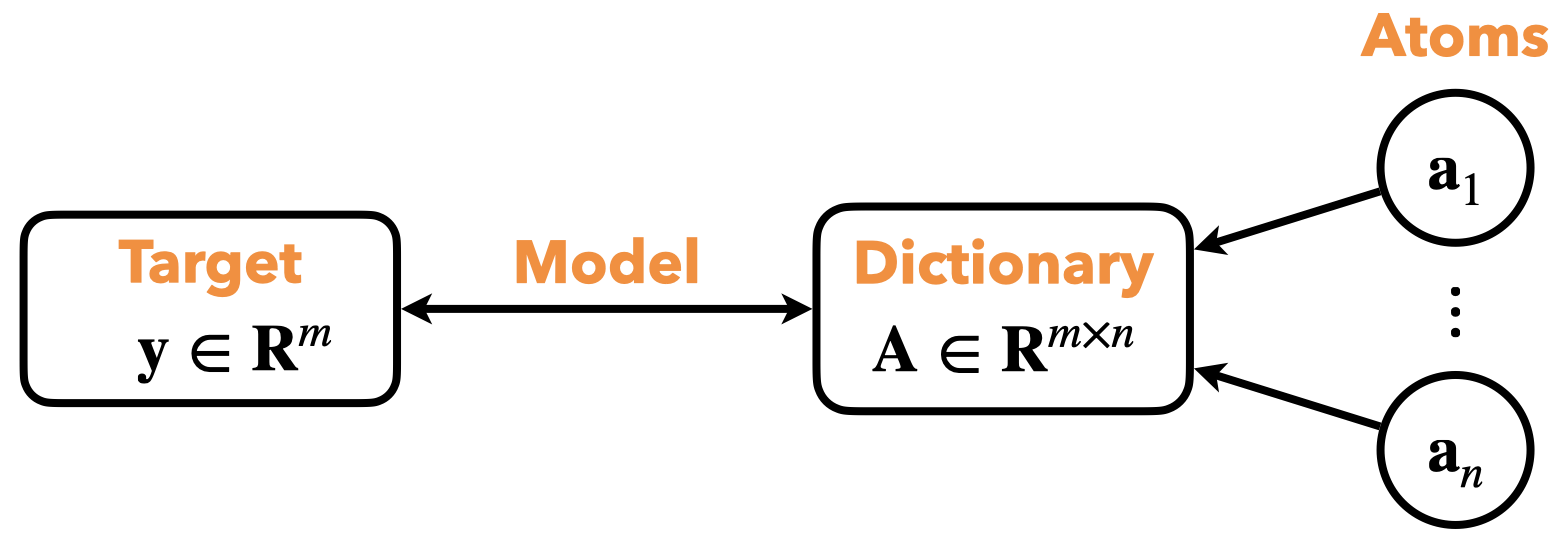
\includegraphics[width=0.9\linewidth]{Illustrations/Illustrations.001.png}
  \end{center}
\end{frame}

\begin{frame}{Sparse problems}
  \textbf{Objective :} \emphone{Fit} the target with a \emphone{sparse} combination of atoms
  \vspace*{0.5cm}
  \begin{center}
    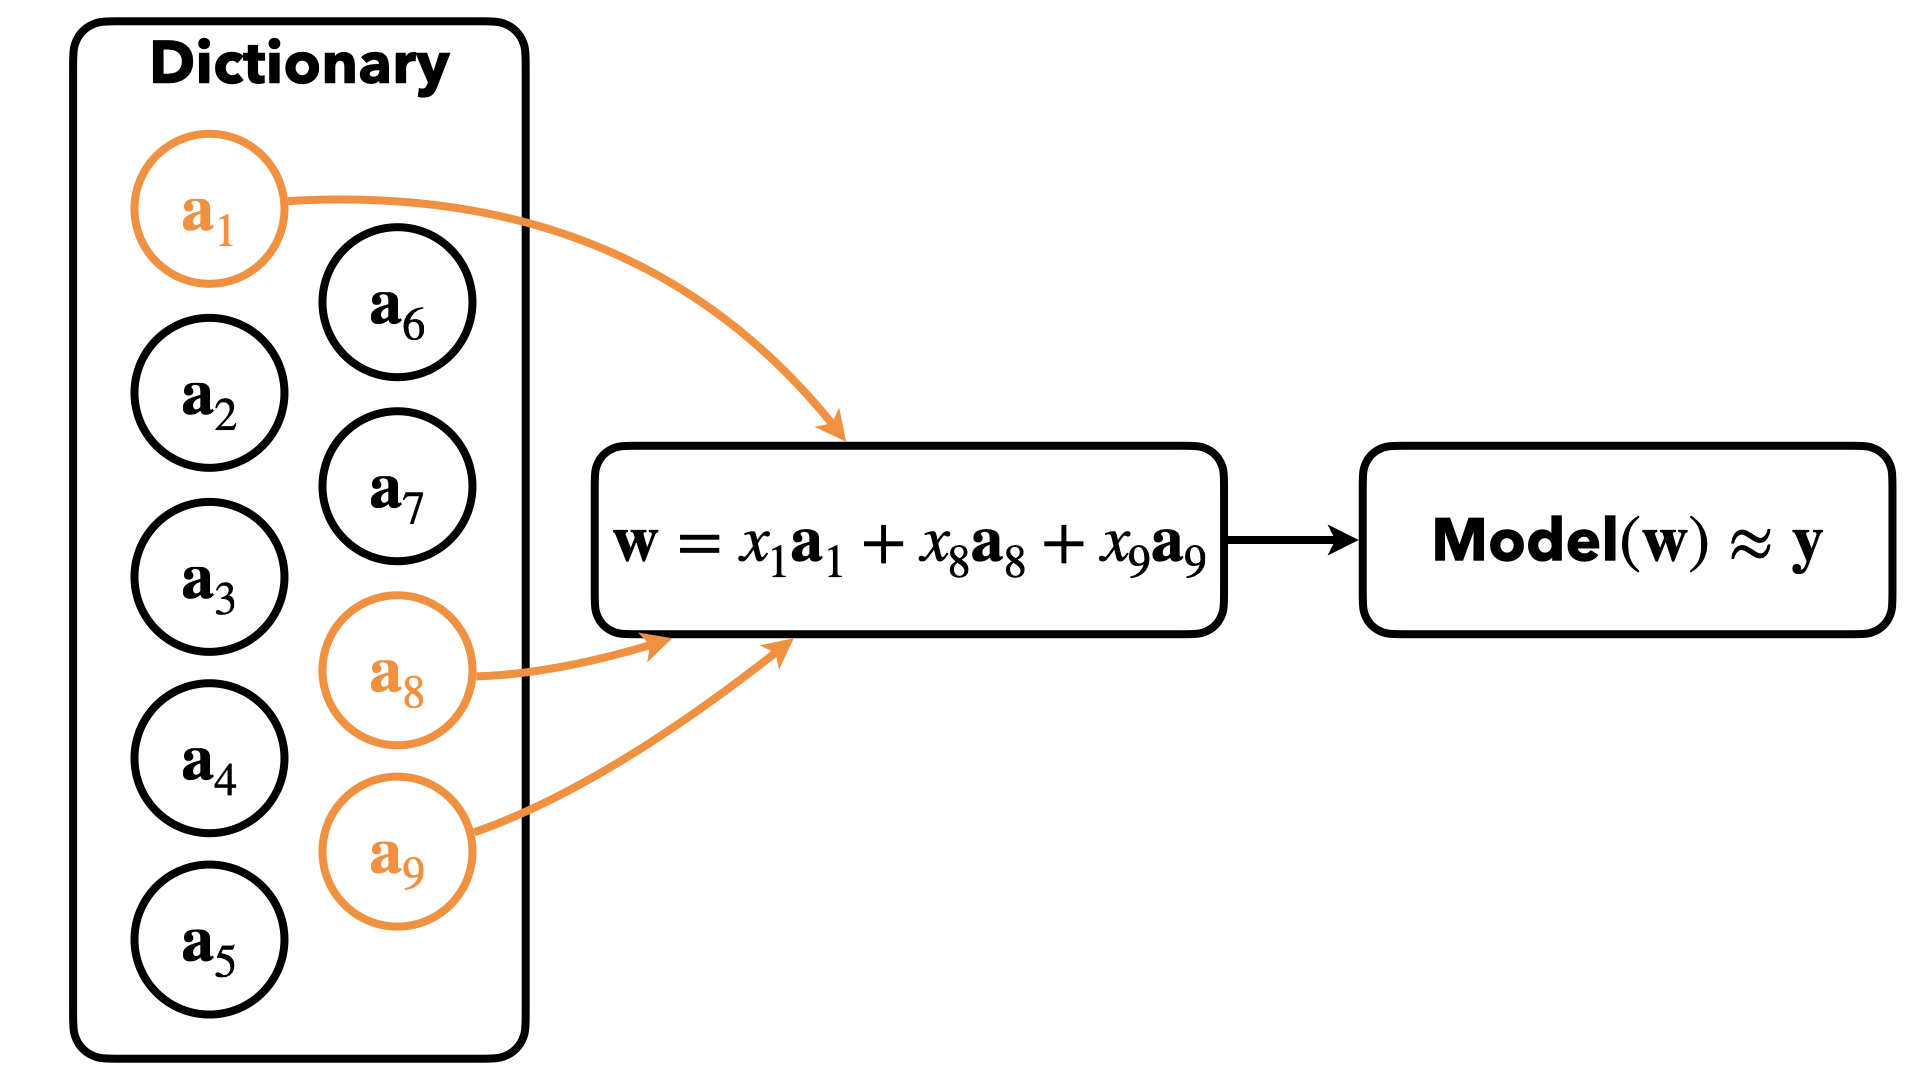
\includegraphics[width=0.8\linewidth]{Illustrations/Illustrations.002.png}
  \end{center}
\end{frame}

\begin{frame}{Sparse problems}
  \begin{center}
    \begin{minipage}{0.6\linewidth}
      \begin{block}{Rough formulation}
        \centering
        Find \emphone{$\pv$ sparse} such that \emphone{$\obs \simeq$ Model$(\dic \pv)$}
      \end{block}
    \end{minipage}
  \end{center}
  \pause
  \begin{center}
    \emph{Remark : Entries in $\pv$ weight each atom in the dictionary.}
  \end{center}
  \pause
  \begin{center}
    \rotatebox[origin=c]{-90}{\LARGE$\leadsto$}
  \end{center}
  \vspace*{-0.5cm}
  \begin{center}
    \begin{minipage}{0.6\linewidth}
      \begin{block}{$\ell_0$-penalized problem}
        \begin{equation}
          \label{prob:prob} 
          \tag{\(\ppb\)}
          \optobj = \min \datafunc(\obs,\dic\pv) + \reg \norm{\pv}{0}
        \end{equation}
      \end{block}
    \end{minipage}
  \end{center}
  \pause
  \begin{itemize}
    \item $\datafunc$ ensures the \emphone{model fitting}
    \item $\norm{\cdot}{0}$ enforces \emphone{sparsity}
    \item $\reg>0$ controls the \emphone{trade-off}
  \end{itemize}
  \pause
  \begin{center}
    \emphone{\eqref{prob:prob} \textbf{is NP-hard !}}
  \end{center}
\end{frame}

% \begin{frame}{Sparse problems}
%   \textbf{A signal processing example}
%   \pause
%   \begin{center}
%     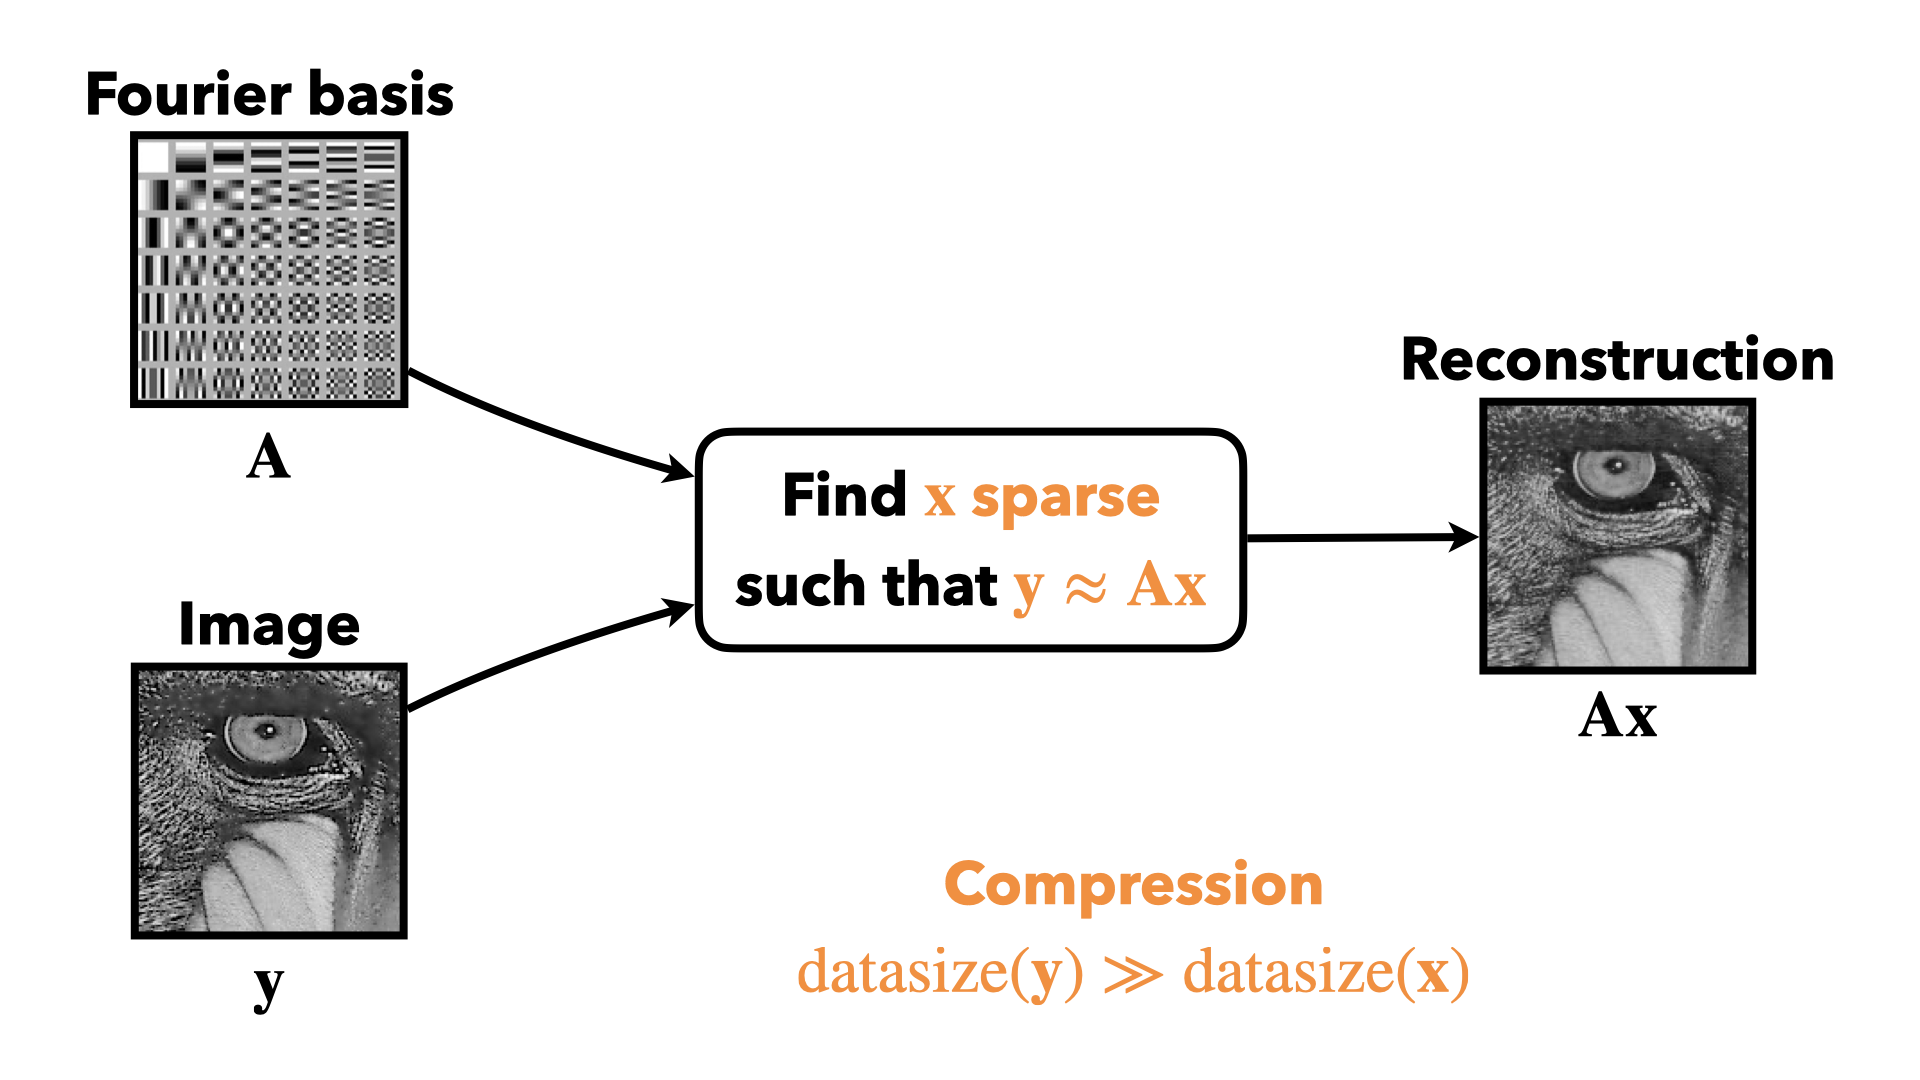
\includegraphics[width=\linewidth]{Illustrations/Illustrations.003.png}
%   \end{center}
% \end{frame}

% \begin{frame}{Sparse problems}
%   \textbf{A machine learning example}
%   \pause
%   \begin{center}
%     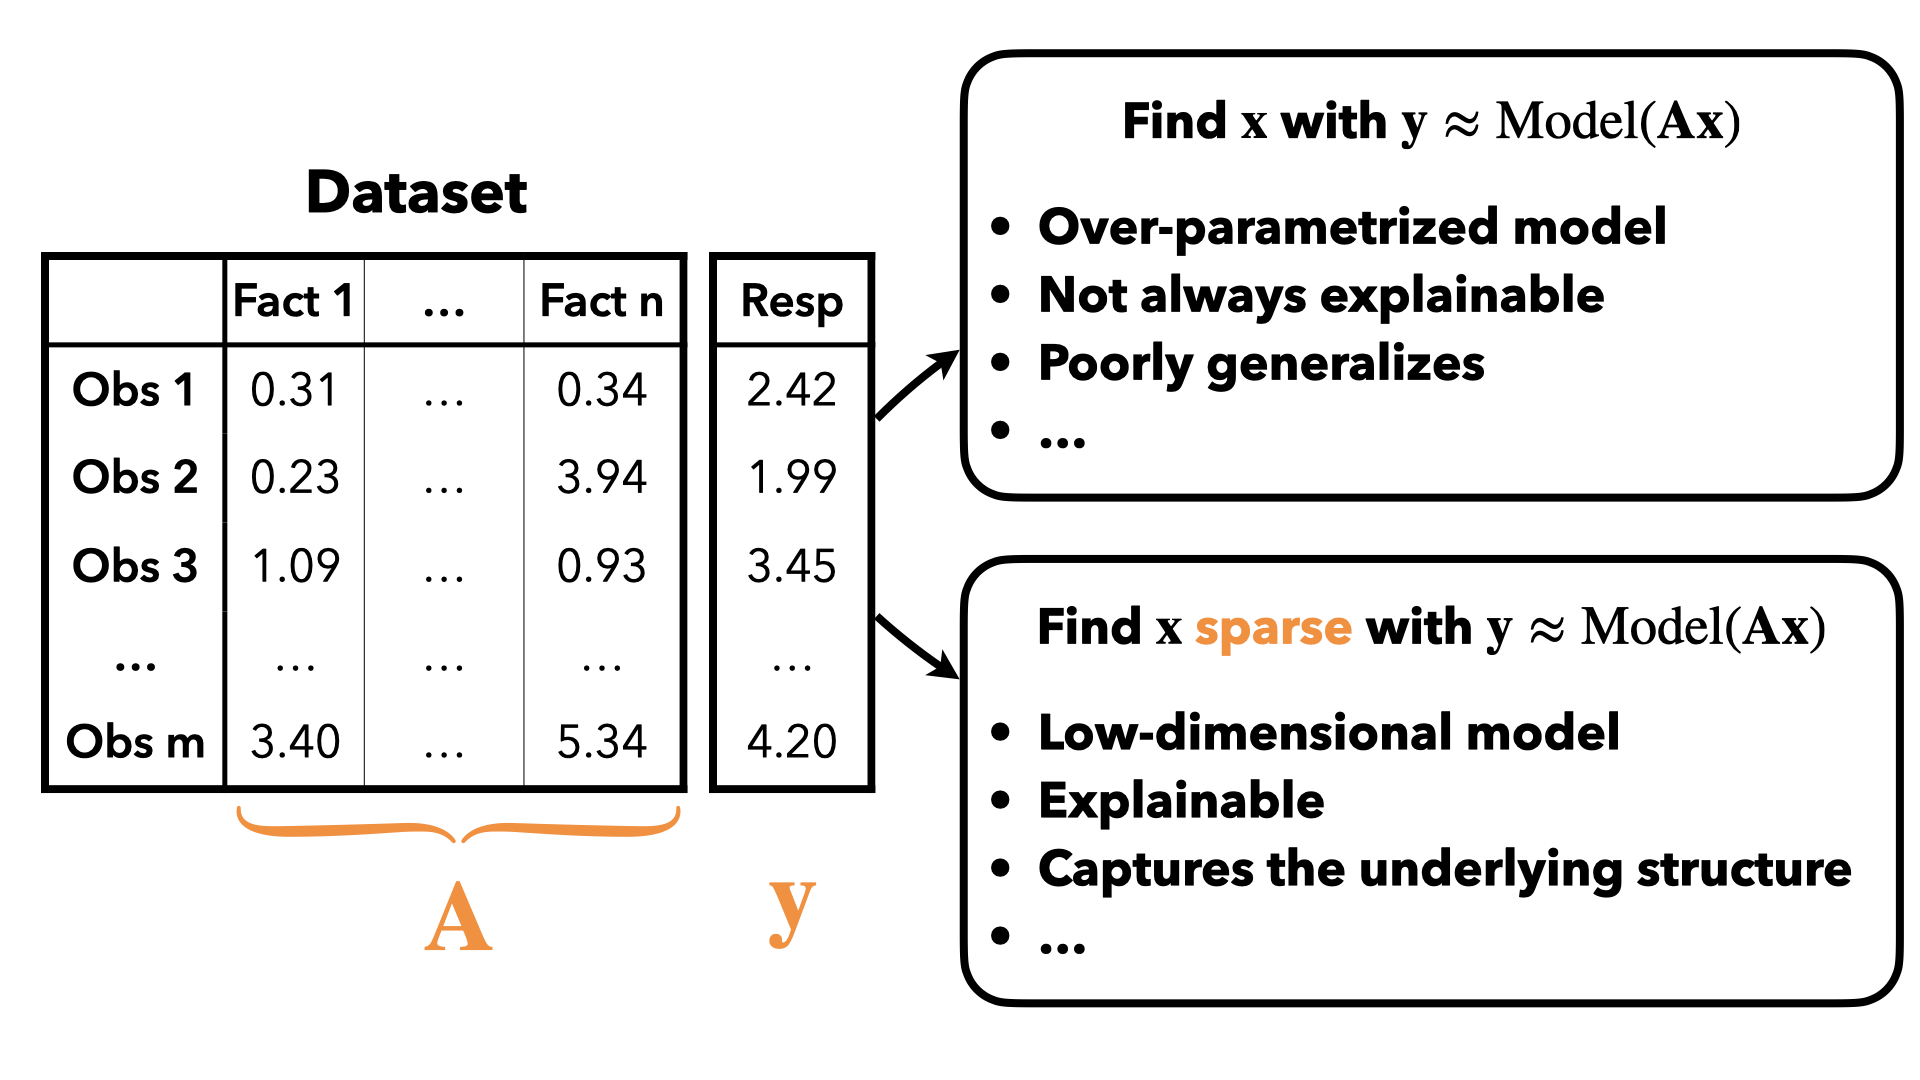
\includegraphics[width=\linewidth]{Illustrations/Illustrations.004.png}
%   \end{center}
% \end{frame}

\section{\gls{mip} formulation}

\begin{frame}{\gls{mip} formulations}
  \textbf{\gls{mip}}
  \begin{itemize}
    \item Optimization problem
    \item Objective and constraints
    \item Continuous and integer variables
  \end{itemize}
  \pause
  \textbf{Solver friendly structures}
  \begin{itemize}
    \item Linear and quadratic expressions (GLPK, Cbc, CPLEX, Gurobi, ...)
    \item Conic expressions (Knitro, Mosek, ...)
    \item Non-linear expressions (Couenne, ...)
  \end{itemize}
  \pause
  \begin{center}
    \emphone{\textbf{The $\ell_0$-norm is not solver friendly !}}
  \end{center}
\end{frame}

\section{\gls{sos} approach}

\begin{frame}{\gls{sos} approach}
  
  \begin{textblock*}{100pt}(265pt,25pt)
    \scriptsize{
      \begin{equation}
        \nonumber
        \norm{\pvi{}}{0} =
        \begin{cases}
          0 &\text{if} \ \pvi{} = 0 \\
          1 &\text{if} \ \pvi{} \neq 0
        \end{cases}
      \end{equation}
    }
  \end{textblock*}

  \textbf{Idea :} Model the \emphone{nullity} in $\pv$ using a \emphone{binary} variable.
  \pause
  \vspace*{0.5cm}
  \begin{block}{Modelling nullity in $\pv$}
    Let $\bv \in \{0,1\}$, then the constraint
    \begin{equation}
      \emphone{\pv(1-\bv) = 0 \iff (\pv,\bv) \in SOS_1} \nonumber
    \end{equation}
    models the nullity in $\pv$ entries.
  \end{block}
  \pause
  \textbf{Solver friendly formulation}
  \begin{equation}
    \label{prob:prob-SOS} 
    \tag{\(\ppb_{sos}\)}
    \optobj = \left\{
      \begin{array}{rl}
        \min & \datafunc(\obs,\dic\pv) + \reg \emphone{\transp{\1}\bv} \\ 
        \st & \emphone{(\pv,\bv) \in SOS_1} \\ & \pv \in \kR^{\pdim}, \ \bv \in \{0,1\}^{\pdim}
      \end{array}
    \right.
  \end{equation}
\end{frame}

\begin{frame}{\gls{sos} approach}
  \begin{center}
    
\includegraphics[width=\linewidth]{Illustrations/Illustrations.005.png}
  \end{center}
  \pause
  \begin{minipage}[t]{0.49\linewidth}
    \textbf{Pros}
    \begin{itemize}
      \item[\ding{51}] Standard formulation 
      \item[\ding{51}] Explicitly models sparsity
      \item[\ding{51}] Simple
    \end{itemize}
  \end{minipage}
  \hfill
  \pause
  \begin{minipage}[t]{0.49\linewidth}
    \textbf{Cons}
    \begin{itemize}
      \item[\ding{55}] Twice more variables
      \item[\ding{55}] Handling \texttt{SOS}${}_1$ constraints
      \item[\ding{55}] New layer of complexity
    \end{itemize}
  \end{minipage}
\end{frame}

\section{\gls{bnb} approach}

\begin{frame}{\gls{bnb} approach}
  \textbf{\gls{bnb} algorithms}
  \begin{itemize}
    \item Separation of the search space
    \item Enumerate all feasible solutions
    \item Use rules to discard irrelevant candidates
    \item[$\rightarrow$] Explore a \emphone{decision tree} and \emphone{prune} uninteresting \emphone{nodes}
  \end{itemize}
  \pause
  \textbf{Particularization to \eqref{prob:prob}}
  \begin{itemize}
    \item Node defined as $\nodeSymb = (\setzero,\setone,\setnone)$
    \begin{itemize}
      \item $\setzero$ : indices of $\pv$ fixed to \emphone{zero}
      \item $\setone$ : indices of $\pv$ fixed to \emphone{non-zero}
      \item $\setnone$ : indices of $\pv$ \emphone{not fixed yet}
    \end{itemize}
    \item Decisions about the nullity in the problem variable
  \end{itemize}
\end{frame}

\begin{frame}{\gls{bnb} approach}
  \only<1>{
    \begin{figure}
      \forestset{
    node/.style = {
        draw, 
        circle,
        thick,
        align = center,
        font = \small,
        top color = white,
        bottom color = teal!50,
    },
    branch label/.style={
        edge label = {
            node[midway,fill=white,font=\small,draw=black,text height=0.5em,scale=0.9]{#1}
        }
    },
    bnb/.style={
        branch label,
        for tree = {
            node,
            s sep'+=14mm,
            l sep'+=2mm,
            edge={->},
            edge+={thick},
        },
        before typesetting nodes={
            for tree={
                split option={content}{:}{content,branch label},
            },
        },
        where n children=0{
            tikz+={
                \draw [thick,dashed,->]  ([yshift=0pt, xshift=0pt].south east) -- ([yshift=-5pt, xshift=5pt].south east);
                \draw [thick,dashed,->]  ([yshift=0pt, xshift=0pt].south west) -- ([yshift=-5pt, xshift=-5pt].south west);
            }
        }{},
    },
}
\begin{forest}
    bnb,
    [
        \(\nodeSymbIter{0}\)
            [\(\nodeSymbIter{1}\):\({\pvi{\idxentrynode_1}=0}\)
            [\(\nodeSymbIter{3}\):\({\pvi{\idxentrynode_2}=0}\)]
            [\(\nodeSymbIter{4}\):\({\pvi{\idxentrynode_2}\neq0}\)]
    ][
        \(\nodeSymbIter{2}\):\({\pvi{\idxentrynode_1}\neq0}\),
            [\(\nodeSymbIter{5}\):\({\pvi{\idxentrynode_2}=0}\)]
            [\(\nodeSymbIter{6}\):\({\pvi{\idxentrynode_2}\neq0}\)]
    ]
    ]
\end{forest}
      \caption{Example of \gls{bnb} tree.}
    \end{figure}
  }
  \only<2>{
    \begin{figure}
      \forestset{
    node/.style = {
        draw, 
        circle,
        thick,
        align = center,
        font = \small,
        top color = white,
        bottom color = teal!50,
    },
    branch label/.style={
        edge label = {
            node[midway,fill=white,font=\small,draw=black,text height=0.5em,scale=0.9]{#1}
        }
    },
    bnb/.style={
        branch label,
        for tree = {
            node,
            s sep'+=14mm,
            l sep'+=2mm,
            edge={->},
            edge+={thick},
        },
        before typesetting nodes={
            for tree={
                split option={content}{:}{content,branch label},
            },
        },
    },
}
\begin{forest}
    bnb,
    [
        \(\nodeSymbIter{0}\)
            [\(\nodeSymbIter{1}\):\({\pvi{\idxentrynode_1}=0}\)
            [\(\nodeSymbIter{3}\):\({\pvi{\idxentrynode_2}=0}\)] {
                \draw [thick,dashed,->] ([yshift=0pt, xshift=0pt].south east) -- ([yshift=-5pt, xshift=5pt].south east);
                \draw [thick,dashed,->]  ([yshift=0pt, xshift=0pt].south west) -- ([yshift=-5pt, xshift=-5pt].south west);
            }
            [\(\nodeSymbIter{4}\):\({\pvi{\idxentrynode_2}\neq0}\),bottom color = red!50]
    ][
        \(\nodeSymbIter{2}\):\({\pvi{\idxentrynode_1}\neq0}\),
            [\(\nodeSymbIter{5}\):\({\pvi{\idxentrynode_2}=0}\),bottom color = red!50]
            [\(\nodeSymbIter{6}\):\({\pvi{\idxentrynode_2}\neq0}\),bottom color = red!50]
    ]
    ]
\end{forest}
      \caption{Example of \gls{bnb} tree.}
    \end{figure}
  }
\end{frame}

\begin{frame}{\gls{bnb} approach}

  \textbf{Node $\nodeSymb=(\setzero,\setone,\setnone)$ :} Does a solution of \eqref{prob:prob} match the constraints ? 

  \pause
  \vspace{0.2cm}

  \begin{block}{Problem at node $\nodeSymb$}
    \begin{equation}
      \label{prob:prob-node} \tag{\(\node{\ppb}\)}
      \node{\pobj} \ =
      \left\{
      \begin{array}{rl}
        \min & \datafunc(\obs,\dic\pv) + \reg \norm{\pv}{0} \\
        \st & \emphone{\subzero{\pv} = \0, \ \subone{\pv} \neq \0}
      \end{array}
      \right.
    \end{equation}
    If \emphone{$\opt{\pobj} < \node{\pobj}$}, then node $\nodeSymb$ can be \emphone{pruned} from the \gls{bnb} tree.
  \end{block}

  \vspace*{1cm}
  \pause
  \textbf{Practical issue :}
  Neither $\opt{\pobj}$ nor $\node{\pobj}$ are accessible in practice.
  \pause
  \begin{center}
    \begin{tikzpicture}
    \draw[thick,->] (0,0) -- (6,0);
    \node at (6.5,0.05) (axis_text) {value};

    \node at (0.5,0) (opt) {};
    \draw[thick,red] (opt.north) -- (opt.south);
    \node[red] at (0.5,-0.4) (opt_text) {$\opt{\pobj}$};

    \node at (4,0) (pv1) {};
    \draw[thick,teal] (pv1.north) -- (pv1.south);
    \node[teal] at (4,-0.4) (pv1_text) {$\node{\pobj}$};

    \pause
    \node at (1.5,0) (ub) {};
    \draw[thick,red,->] (opt) .. controls (1,0.5) and (1,0.5) .. (ub);
    \node[red] at (1,0.6) (opt_arrow_text) {\scriptsize restriction};
    \draw[thick,red] (ub.north) -- (ub.south);
    \node[red] at (1.5,-0.4) (ub_text) {$\UB{\pobj}$};

    \pause
    \node at (2,0) (dv1) {};
    \draw[thick,teal] (dv1.north) -- (dv1.south);
    \node[teal] at (2,-0.4) (dv1_text) {$\node{\robj}$};
    \draw[thick,teal,->] (pv1) .. controls (3,0.5) and (3,0.5) .. (dv1);
    \node[teal] at (3,0.6) (dv1_arrow_text) {\scriptsize relaxation};

\end{tikzpicture}
  \end{center}
\end{frame}

\begin{frame}{\gls{bnb} approach}
  \textbf{Finding some \emphone{upper} bound $\UB{\pobj} \geq \opt{\pobj}$}
  \begin{itemize}
    \item Keep track of the best objective value known for \eqref{prob:prob}
    \item Refine $\UB{\pobj}$ using heuristics during the tree exploration
  \end{itemize}
  \vspace*{0.5cm}
  \pause
  \textbf{Finding some \emphone{lower} bound $\node{\robj} \leq \node{\pobj}$}
  \begin{itemize}
    \item Relax the objective function of \eqref{prob:prob-node} into a \emphone{convex} function
  \end{itemize}
\end{frame}

\begin{frame}{\gls{bnb} approach}
  \textbf{Relaxing the $\ell_0$-norm at $\nodeSymb=(\setzero,\setone,\setnone)$} \\
  \pause
  \begin{itemize}
    \item[$\rightarrow$] \emphone{Separable}
    \pause
    \item[$\rightarrow$] \emphone{Closed-form} expression for indices in $\setzero$ or $\setone$
  \end{itemize}
  \pause
  \begin{equation}
    \nonumber
    \norm{\pv}{0} = \underbrace{\norm{\subzero{\pv}}{0}}_{\emphone{0}} + \underbrace{\norm{\subone{\pv}}{0}}_{\emphone{\card{\setone}}} + \norm{\subnone{\pv}}{0}
  \end{equation}
  \vspace*{0.5cm}
  ~\\
  \pause
  \newcommand{\pointsize}{0.04}
\begin{figure}[!ht]
  \small
  \begin{tikzpicture}[
      domain=-1:1,
      xscale = 2,
      yscale = 2,
      lbl/.style = {font=\scriptsize, fill=white, 
      inner sep=2pt}
  ]
    \node (origin) at (0,0) {};
    \draw[->] (-1,0) -- (1, 0);
    \draw[->] (0,0) -- (0, 1);
    \draw (-0.03, 0.75) -- (0.03, 0.75);
    \node[above right] at (0,0.75) {$1$};
    \node[right] at (1,0) {$\pv$};
    \draw[-{Arc Barb[arc=180,reversed]},teal,thick] (-0.75, 0.75) -- (-0.01, 0.75);
    \draw[teal,thick,dashed] (-1.2, 0.75) -- (-0.75, 0.75);
    \draw[{Arc Barb[arc=180,reversed]}-,teal,thick] (0.01, 0.75) -- (0.75, 0.75);
    \draw[teal,thick,dashed] (0.75, 0.75) -- (1.2, 0.75);
    \node[right,teal] at (1.2,0.75) {$\norm{\pv}{0}$};
    \fill[teal] (0,0) circle (\pointsize);
    \draw[red,thick] (-1, 0.85) .. controls (0, -0.5) and (0, -0.5) .. (1, 0.85);
  \end{tikzpicture}
\end{figure}
  \pause
  \vspace*{-0.5cm}
  \begin{center}
    \textbf{\emphone{No valid convex relaxation !}}
  \end{center}
\end{frame}

\begin{frame}{\gls{bnb} approach}
  \begin{center}
    \begin{minipage}{0.7\linewidth}
      \begin{block}{\emphone{Perturbated} $\ell_0$-penalized problem}
        Rather consider
        \begin{equation}
          \label{prob:prob-pertrbated} 
          \tag{\(\ppb_{\pertfunc}\)}
          \optobj = \min \datafunc(\obs,\dic\pv) + \reg (\emphone{\norm{\pv}{0} + \pertfunc(\pv)})
        \end{equation}
        where $\pertfunc(\cdot)$ is a convex function.
      \end{block}
    \end{minipage}
  \end{center}
  \pause
  \vspace*{1cm}
  \begin{minipage}[t]{0.49\linewidth}
    \textbf{Case $\pertfunc(\pv)= \Icvx(\norm{\pv}{\infty} \leq \bigM)$} 
    \pause
    \vspace*{0.05cm}
    \newcommand{\pointsize}{0.04}
\begin{figure}[!ht]
  \small
  \begin{tikzpicture}[
      domain=-0.8:0.8,
      xscale = 2,
      yscale = 2,
      lbl/.style = {font=\scriptsize, fill=white, 
      inner sep=2pt}
  ]
    \node (origin) at (0,0) {};
    \draw[->] (-1,0) -- (1, 0);
    \draw[->] (0,0) -- (0, 1);
    \draw (-0.03, 0.3) -- (0.03, 0.3);
    \node[above right] at (0,0.3) {$1$};
    \node[right] at (1, 0) {$\pv$};
    \draw[-{Arc Barb[arc=180,reversed]},teal,thick] (-0.5, 0.3) -- (-0.01, 0.3);
    \draw[{Arc Barb[arc=180,reversed]}-,teal,thick] (0.01, 0.3) -- (0.5, 0.3);
    \fill[teal] (0,0) circle (\pointsize);
    \draw (-0.5, 0.03) -- (-0.5, -0.03);
    \draw (0.5, 0.03) -- (0.5, -0.03);
    \node[below] at (-0.5, 0) {-$\bigM$};
    \node[below] at (0.5, 0) {$\bigM$};
    \pause
    \draw (-0.03, 0.8) -- (0.03, 0.8);
    \node[right] at (0,0.8) {$+\infty$};
    \draw[teal,thick,dashed] (-0.5, 0.8) -- (-0.8, 0.8);
    \draw[teal,thick,dashed] (0.5, 0.8) -- (0.8, 0.8);
    \node[above,teal] at (1.17,0.8) {$\norm{\pv}{0} + \pertfunc(\pv)$};
    \pause
    \draw[red,thick] (0, 0) -- (0.515, 0.3);
    \draw[red,thick] (0, 0) -- (-0.515, 0.3);
    \draw[red,thick,dashed] (-0.5, 0.785) -- (-0.8, 0.785);
    \draw[red,thick,dashed] (0.5, 0.785) -- (0.8, 0.785);
    \fill[teal] (0,0) circle (\pointsize);
  \end{tikzpicture}
\end{figure}
  \end{minipage}
  \hfill
  \begin{minipage}[t]{0.49\linewidth}
    %
  \end{minipage}
\end{frame}

\begin{frame}{\gls{bnb} approach}
  \begin{center}
    \begin{minipage}{0.7\linewidth}
      \begin{block}{\emphone{Perturbated} $\ell_0$-penalized problem}
        Rather consider
        \begin{equation}
          \label{prob:prob-pertrbated} 
          \tag{\(\ppb_{\pertfunc}\)}
          \optobj = \min \datafunc(\obs,\dic\pv) + \reg (\emphone{\norm{\pv}{0} + \pertfunc(\pv)})
        \end{equation}
        where $\pertfunc(\cdot)$ is a convex function.
      \end{block}
    \end{minipage}
  \end{center}
  \vspace*{1cm}
  \mytransparentbox{
    \begin{minipage}[t]{0.49\linewidth}
      \textbf{Case $\pertfunc(\pv)= \Icvx(\norm{\pv}{\infty} \leq \bigM)$} 
      \vspace*{0.05cm}
      \newcommand{\pointsize}{0.04}
\begin{figure}[!ht]
  \small
  \begin{tikzpicture}[
      domain=-0.8:0.8,
      xscale = 2,
      yscale = 2,
      lbl/.style = {font=\scriptsize, fill=white, 
      inner sep=2pt}
  ]
    \node (origin) at (0,0) {};
    \draw[->,opacity=0.5] (-1,0) -- (1, 0);
    \draw[->,opacity=0.5] (0,0) -- (0, 1);
    \draw[opacity=0.5] (-0.03, 0.3) -- (0.03, 0.3);
    \node[above right] at (0,0.3) {$1$};
    \node[right] at (1, 0) {$\pv$};
    \draw[-{Arc Barb[arc=180,reversed]},teal,thick,opacity=0.5] (-0.5, 0.3) -- (-0.01, 0.3);
    \draw[{Arc Barb[arc=180,reversed]}-,teal,thick,opacity=0.5] (0.01, 0.3) -- (0.5, 0.3);
    \fill[teal] (0,0) circle (\pointsize);
    \draw[opacity=0.5] (-0.5, 0.03) -- (-0.5, -0.03);
    \draw[opacity=0.5] (0.5, 0.03) -- (0.5, -0.03);
    \node[below] at (-0.5, 0) {-$\bigM$};
    \node[below] at (0.5, 0) {$\bigM$};
    \draw[opacity=0.5] (-0.03, 0.8) -- (0.03, 0.8);
    \node[right] at (0,0.8) {$+\infty$};
    \draw[teal,thick,dashed,opacity=0.5] (-0.5, 0.8) -- (-0.8, 0.8);
    \draw[teal,thick,dashed,opacity=0.5] (0.5, 0.8) -- (0.8, 0.8);
    \node[above,teal] at (1.17,0.8) {$\norm{\pv}{0} + \pertfunc(\pv)$};
    \draw[red,thick,opacity=0.5] (0, 0) -- (0.515, 0.3);
    \draw[red,thick,opacity=0.5] (0, 0) -- (-0.515, 0.3);
    \draw[red,thick,dashed,opacity=0.5] (-0.5, 0.785) -- (-0.8, 0.785);
    \draw[red,thick,dashed,opacity=0.5] (0.5, 0.785) -- (0.8, 0.785);
    \fill[teal] (0,0) circle (\pointsize);
  \end{tikzpicture}
\end{figure}
    \end{minipage}
  }
  \hfill
  \begin{minipage}[t]{0.49\linewidth}
    \textbf{Case $\pertfunc(\pv)= \alpha\norm{\pv}{2}^2$} 
    \pause
    \newcommand{\pointsize}{0.04}
\begin{figure}[!ht]
  \small
  \begin{tikzpicture}[
      domain=-0.8:0.8,
      xscale = 2,
      yscale = 2,
      lbl/.style = {font=\scriptsize, fill=white, 
      inner sep=2pt}
  ]
    \node (origin) at (0,0) {};
    \draw[->] (-1,0) -- (1, 0);
    \draw[->] (0,0) -- (0, 1);
    \draw (-0.03, 0.3) -- (0.03, 0.3);
    \node[above right] at (0,0.3) {$1$};
    \node[right] at (1, 0) {$\pv$};
    \draw[{Arc Barb[arc=180,reversed]}-,teal,thick] (-0.5,0.3) plot[domain=0.01:0.8] (\x,0.3+\x^2) node[anchor=west] {$\norm{\pv}{0} + \pertfunc(\pv)$};
    \draw[-{Arc Barb[arc=180,reversed]},teal,thick] (-0.5,0.3) plot[domain=-0.8:-0.01] (\x,0.3-\x^2) node {};
    \fill[teal] (0,0) circle (\pointsize);
    \pause
    \draw[red,thick] (0, 0) -- (0.5, 0.53);
    \draw[red,thick] (0.5, 0.53) plot[domain=0.5:0.8] (\x,0.3+\x^2-0.02) node {};
    \draw[red,thick] (0, 0) -- (-0.5, 0.53);
    \draw[red,thick] (-0.5, 0.53) plot[domain=-0.8:-0.5] (\x,0.3-\x^2-0.02) node {};
    \fill[teal] (0,0) circle (\pointsize);
  \end{tikzpicture}
\end{figure}
  \end{minipage}
\end{frame}

\begin{frame}{\gls{bnb} approach}
  \textbf{Explore less and faster}
  \pause
  \begin{itemize}
    \item \emphone{Coordinate Descent} to solve the relaxations \emph{(Hazimeh \etal, 2021)}
    \pause
    \item \emphone{Screening} to accelerate the CD \emph{(El Ghaoui \etal, 2011)}
    \pause
    \item \emphone{Node-screening} to discard uninteresting nodes \emph{(Guyard \etal, 2022)}
    \pause
    \item \emphone{Early pruning} to save computations \emph{(Samain \etal, 2022)}
    \pause
    \item ...
  \end{itemize}
\end{frame}

\begin{frame}{\gls{bnb} approach}
  \begin{center}
    
\includegraphics[width=\linewidth]{Illustrations/Illustrations.006.png}
  \end{center}
  \pause
  \begin{minipage}[t]{0.49\linewidth}
    \textbf{Pros}
    \begin{itemize}
      \item[\ding{51}] Tailored \gls{bnb} algorithm 
      \item[\ding{51}] Exploit sparsity
      \item[\ding{51}] Faster convergence
    \end{itemize}
  \end{minipage}
  \hfill
  \pause
  \begin{minipage}[t]{0.49\linewidth}
    \textbf{Cons}
    \begin{itemize}
      \item[\ding{55}] Perturb the problem
      \item[\ding{55}] New hyperparameters to tune
    \end{itemize}
  \end{minipage}
\end{frame}

\begin{frame}
  \begin{center}
    \LARGE\textbf{\emphone{Conclusion}}
  \end{center}
  \pause
  \vspace*{0.5cm}
  \textbf{Addressing $\ell_0$-penalized problems}
  \pause
  \vspace*{0.3cm}
  \begin{itemize}
    \item Leveraging \texttt{SOS}${}_1$ constraints
    \begin{itemize}
      \item[\ding{51}] MIP formulation
      \item[\ding{51}] Generic solvers
      \item[\ding{55}] Still hard to handle
    \end{itemize}
    \pause
    \vspace*{0.5cm}
    \item Using a Branch-and-Bound procedure
    \begin{itemize}
      \item[\ding{51}] Specialized solution method
      \item[\ding{51}] Efficient to solve the problem
      \item[\ding{55}] Have to perturb the problem
    \end{itemize}
  \end{itemize}
\end{frame}

\setbeamercolor{frametitle}{fg=white,bg=mLightBrown}
\begin{frame}[fragile]{Advertizing time}
  \begin{center}
    \url{https://github.com/TheoGuyard/El0ps.jl}
%     ~\\
%     \pause
%     \vspace*{1cm}
%     \begin{minipage}{0.7\linewidth}
%       \begin{lstlisting}
% using El0ps
% using CPLEX

% # ... set problem data

% problem = Problem(F,G,A,y,lmbd)
% solver  = DirectSolver(CPLEX.Optimizer)
% solver  = BnbSolver()
% optimize(solver,problem)
%       \end{lstlisting}
%     \end{minipage}
  \end{center}
\end{frame}

% \section{Numerical illustrations}

% \begin{frame}{Synthetic data generation}

% \end{frame}

% \section{Branch-and-bound algorithms}

% \begin{frame}{Branch-and-bound principle}
%   \textbf{Idea :}
%   \begin{itemize}
%     \item Enumerate all feasible solutions
%     \pause
%     \item Use tests to discard irrelevant candidates
%     \pause
%     \item[$\rightarrow$] \emphone{Explore a decision tree and prune uninteresting nodes} 
%   \end{itemize}

%   \pause

%   \textbf{Node} $\nodeSymb = (\setzero,\setone,\setnone)$ \textbf{where :}
%   \begin{itemize}
%     \item $\setzero$ : indices of $\pv$ fixed to \emphone{zero}
%     \item $\setone$ : indices of $\pv$ fixed to \emphone{non-zero}
%     \item $\setnone \ $ : indices not fixed yet
%   \end{itemize}

%   \pause

%   \begin{figure}
%     \centering
%     \scalebox{0.7}{\input{img/bnb}}
%   \end{figure}
% \end{frame}

% \begin{frame}{Processing node $\nodeSymb = (\setzero,\setone,\setnone)$}

%   \textbf{Question :} Does any solution of \eqref{prob:prob} match the current constraints ? 

%   \pause
%   \vspace{0.2cm}

%   \begin{block}{\emphone{Sub}-problem at node $\nodeSymb$}
%     \begin{equation}
%       \label{prob:prob-node} \tag{\(\node{\mpb}\)}
%       \node{\pobj} \ =
%       \left\{
%       \begin{array}{rl}
%         \min & \datafunc(\dic\pv) + \reg \norm{\pv}{0}\\
%         \text{s.t.} & \kvvbar{\pv}_{\infty} \leq \bigM
%       \end{array}
%       \right\}
%       \bigcap
%       \emphone{
%       \left\{
%       \begin{array}{rl}
%         \subzero{\pv} &= \0 \\
%         \subone{\pv} &\neq \0
%       \end{array}
%       \right\}
%       }
%     \end{equation}
%     If \emphone{$\opt{\pobj} < \node{\pobj}$}, then node $\nodeSymb$ can be \emphone{pruned} from the \gls{bnb} tree.
%   \end{block}

%   \pause
%   Neither $\opt{\pobj}$ nor $\node{\pobj}$ are accessible in practice :
%   \pause
%   \begin{itemize}
%     \item \emphone{Restriction} : Upper bound $\UB{\pobj}$ on $\opt{\pobj}$ \\
%     \pause
%     \item \emphone{Relaxation} : Lower bound $\node{\robj}$ on $\node{\pobj}$ \\
%     \pause
%     \item If \emphone{$\UB{\pobj} < \node{\robj}$}, then node $\nodeSymb$ can be \emphone{pruned}
%     \pause 
%     \item Both $\UB{\pobj}$ and $\node{\robj}$ are computed by solving convex problems
%   \end{itemize}

%   \pause
%   \begin{center}
%     \begin{tikzpicture}
    \draw[thick,->] (0,0) -- (6,0);
    \node at (6.5,0.05) (axis_text) {value};

    \node at (0.5,0) (opt) {};
    \draw[thick,red] (opt.north) -- (opt.south);
    \node[red] at (0.5,-0.4) (opt_text) {$\opt{\pobj}$};

    \node at (4,0) (pv1) {};
    \draw[thick,teal] (pv1.north) -- (pv1.south);
    \node[teal] at (4,-0.4) (pv1_text) {$\node{\pobj}$};

    \pause
    \node at (1.5,0) (ub) {};
    \draw[thick,red,->] (opt) .. controls (1,0.5) and (1,0.5) .. (ub);
    \node[red] at (1,0.6) (opt_arrow_text) {\scriptsize restriction};
    \draw[thick,red] (ub.north) -- (ub.south);
    \node[red] at (1.5,-0.4) (ub_text) {$\UB{\pobj}$};

    \pause
    \node at (2,0) (dv1) {};
    \draw[thick,teal] (dv1.north) -- (dv1.south);
    \node[teal] at (2,-0.4) (dv1_text) {$\node{\robj}$};
    \draw[thick,teal,->] (pv1) .. controls (3,0.5) and (3,0.5) .. (dv1);
    \node[teal] at (3,0.6) (dv1_arrow_text) {\scriptsize relaxation};

\end{tikzpicture}
%   \end{center}

% \end{frame}

% \begin{frame}{Exploration and pruning process}
%   \begin{figure}
%     \centering
%     \scalebox{1}{\input{img/bnb}}
%   \end{figure}
% \end{frame}

% \begin{frame}{Exploration and pruning process}
%   \begin{figure}
%     \centering
%     \scalebox{1}{\forestset{
    node/.style = {
        draw, 
        circle,
        thick,
        align = center,
        font = \small,
        top color = white,
        bottom color = teal!50,
    },
    branch label/.style={
        edge label = {
            node[midway,fill=white,font=\small,draw=black,text height=0.5em,scale=0.9]{#1}
        }
    },
    bnb/.style={
        branch label,
        for tree = {
            node,
            s sep'+=14mm,
            l sep'+=2mm,
            edge={->},
            edge+={thick},
        },
        before typesetting nodes={
            for tree={
                split option={content}{:}{content,branch label},
            },
        },
    },
}
\begin{forest}
    bnb,
    [
        \(\nodeSymbIter{0}\)
            [\(\nodeSymbIter{1}\):\({\pvi{\idxentrynode_1}=0}\)
            [\(\nodeSymbIter{3}\):\({\pvi{\idxentrynode_2}=0}\)] {
                \draw [thick,dashed,->] ([yshift=0pt, xshift=0pt].south east) -- ([yshift=-5pt, xshift=5pt].south east);
                \draw [thick,dashed,->]  ([yshift=0pt, xshift=0pt].south west) -- ([yshift=-5pt, xshift=-5pt].south west);
            }
            [\(\nodeSymbIter{4}\):\({\pvi{\idxentrynode_2}\neq0}\),bottom color = red!50]
    ][
        \(\nodeSymbIter{2}\):\({\pvi{\idxentrynode_1}\neq0}\),
            [\(\nodeSymbIter{5}\):\({\pvi{\idxentrynode_2}=0}\),bottom color = red!50]
            [\(\nodeSymbIter{6}\):\({\pvi{\idxentrynode_2}\neq0}\),bottom color = red!50]
    ]
    ]
\end{forest}}
%   \end{figure}
% \end{frame}

% \begin{frame}{\gls{bnb} efficiency}
%   The efficiency of the \gls{bnb} algorithm depends on :
%   \begin{itemize}
%     \item The number of nodes processed
%     \item The ability to process nodes quickly
%   \end{itemize}
%   Node-screening improves both of these things !
% \end{frame}

% \section{Node-screening}

% \begin{frame}{Main idea}

%   \begin{center}
%     Testing if a node can be pruned $\quad\equiv\quad$ Solving convex problems
%   \end{center}
  
%   \begin{textblock*}{100pt}(230pt,110pt)
%     \begin{center}
%       \scriptsize{\textcolor{red}{
%         $\uparrow$ \\
%         This is costly      
%       }}
%     \end{center}
%   \end{textblock*}

%   \begin{textblock*}{100pt}(45pt,110pt)
%     \begin{center}
%       \scriptsize{\textcolor{red}{
%         $\uparrow$ \\
%         Sometimes it is obvious !
%       }}
%     \end{center}
%   \end{textblock*}

%   \vspace*{1cm}

%   \pause
%   \textbf{Question :} How to detect prunable nodes in a more \emphone{economic} way ?
% \end{frame}

% \begin{frame}{Dual problem}

%   \begin{center}
%     \input{img/bnb-node}
%   \end{center}
%   \begin{textblock*}{100pt}(205pt,85pt)
%     \scriptsize{
%       Node $\nodeSymbIter{k} = (\setzero,\setone,\setnone)$ \\
%       $\bullet$ Sub-problem \\
%       $\bullet$ Relaxed problem
%     }
%   \end{textblock*}

%   \pause
  
%   \begin{block}{\emphone{Dual} problem at node $\nodeSymb$}
%     \begin{equation} 
%       \label{prob:dual-node}
%       \tag{$\node{\dpb}$} 
%       \max_{\dv \in \kR^{\ddim}} \ 
%       \Big\{ 
%           \node{\dfunc}(\dv) \triangleq -\conj{\datafunc}(-\dv) - 
%           \sum_{\emphone{\idxentry \in \setnone}} [\pivot{}{}(\ktranspose{\atom}_{\idxentry}\dv)]_+ - 
%           \sum_{\emphone{\idxentry \in \setone}} \pivot{}{}(\ktranspose{\atom}_{\idxentry}\dv)
%       \Big\}
%     \end{equation}
%   \end{block} 

%   \pause

%   \begin{itemize}
%     \item One common term to all nodes
%     \item Terms depending on the current node constraints
%     \pause
%     \item The \emphone{pivot} function is defined as $\pivot{}{}(t) = \bigM |t| - \reg$
%   \end{itemize}
% \end{frame}

% \begin{frame}{Dual objective link}
%   \textbf{Direct consequence :} The dual objective at two consecutive nodes differs from only one term.

%   \pause
%   \vspace{0.2cm}
%   \begin{block}{Dual objective link}
%     At node $\nodeSymb=(\setzero,\setone,\setnone)$, let $\idxentry \in \setnone$. Then $\forall \dv$, 
%     \begin{subequations}
%         \begin{align*}
%             \dfunc^{\emphone{\nodePlusZero{\nodeSymb}{\idxentry}}}(\dv) &= \dfunc^{\emphone{\nodeSymb}}(\dv) + [\pivot{}{}(\ktranspose{\atom}_{\idxentry}\dv)]_+
%             \\
%             \dfunc^{\emphone{\nodePlusOne{\nodeSymb}{\idxentry}}}(\dv) &= \dfunc^{\emphone{\nodeSymb}}(\dv) - [\pivot{}{}(\ktranspose{\atom}_{\idxentry}\dv)]_-
%         \end{align*}
%     \end{subequations}
%   \end{block}

%   \pause
%   \begin{center}
%     \input{img/pruning.tex}
%   \end{center}
% \end{frame}

% \begin{frame}{Node-screening test}

%   \begin{block}{Node-screening test}
%     Given some point $\dv$, 
%     \begin{alignat*}{4}
% 			\node{\dfunc}(\dv) + [\pivot{}{}(\ktranspose{\atom}_{\idxentry}\dv)]_+ & > \UB{\pobj} & \quad\implies\quad & \emphone{\text{Fix} \ \pve_{\idxentry} \neq 0 \ \text{at node} \ \nodeSymb} \\
% 			\node{\dfunc}(\dv) - [\pivot{}{}(\ktranspose{\atom}_{\idxentry}\dv)]_- & > \UB{\pobj} & \quad\implies\quad & \emphone{\text{Fix} \ \pve_{\idxentry} = 0 \ \text{at node} \ \nodeSymb}
% 		\end{alignat*}
%   \end{block}

%   \pause

%   \textbf{Nesting property :} If \emphone{multiple} node-screening tests are passed, the corresponding variables can be fixed \emphone{simultaneously}.
% \end{frame}

% \begin{frame}{Consequence of passing a node-screening test}
%   \begin{figure}
%     \centering
%     \scalebox{1}{\input{img/bnb-l0-screening}}
%   \end{figure}
%   \pause
%   \textbf{Consequence :} Less nodes are explored by the \gls{bnb} algorithm.
% \end{frame}

% \section{Some numerical results}

% \begin{frame}{Some numerical results}
%   \newcommand{\CPLEX}{\texttt{CPLEX}}
%   \newcommand{\BNB}{\texttt{BnB}}
%   \newcommand{\BNBscr}{\texttt{BnB+scr}}
%   \newcommand{\sparsitylevel}{k}

%   \textbf{Synthetic setups :} 
%   \begin{enumerate}
%     \item Sample a synthetic $\dic \in \kR^{\ddim\times\pdim}$ with $(\ddim,\pdim)=(500,1000)$ 
%     \pause
%     \item Generate a $\sparsitylevel$-sparse vector $\opt{\pv}$ with $\sparsitylevel \in \{5,\dots,20\}$
%     \pause
%     \item Set $\obs = \dic \opt{\pv}+$ noise with $10$dB SNR
%     \pause
%     \item Tune $\reg$ and $\bigM$ to (hopefully) recover $\opt{\pv}$ by solving \eqref{prob:prob}
%   \end{enumerate}

%   \pause

%   \vspace*{0.25cm}
%   \begin{figure}
%     \centering
%     \begin{minipage}[t]{0.49\textwidth}
%       \input{img/perf-node}
%     \end{minipage}
%     \hfill
%     \pause
%     \begin{minipage}[t]{0.49\textwidth}
%       \input{img/perf-time}
%     \end{minipage}
%   \end{figure}
% \end{frame}

\end{document}
